\section{Introduction}

Traffic engineering (TE) determines how to route traffic through a network to optimize a network-wide objective. Internet Service Providers (ISPs) use traffic engineering for a variety of objectives that include minimizing congestion hotspots, computing backup routes to accommodate links that fail or are taken down for maintenance, making longer term capacity provisioning decisions, optimizing interdomain transit cost or revenue, and so on \cite{rexford}.

Our focus in this paper is first of these objectives, minimizing congestion, which has received the most amount of attention from researchers as well as network operators \cite{COPE1}, \cite{TeXCP06}, \cite{FortzThorup}, \cite{ObliviousRouting}. The most commonly used optimization objective for TE is to minimize the maximum link utilization (MLU) in the network \cite{COPE1,TeXCP06,MultiTM,ObliviousRouting}. Minimizing MLU has been the mantra of TE research and the minimum MLU TE scheme is considered the optimal scheme.  Other cost functions based on link utilization have also been considered where cost of a link is a convex function of link utilization and the aggregate cost of all links in the network is minimized \cite{MATE1,FortzThorup}.

From an ISP's perspective minimizing the MLU reduces the load on the most congested link in the network. Implicitly, it is expected to improve application performance in the network. Another reason why the minimum MLU  TE scheme is prescribed for ISPs is to help the network cope with an increase in traffic demands. This increase could either be due to future increase in overall network traffic \cite{TeXCP06} or due to short-term unexpected spikes in traffic \cite{COPE1}. Minimizing MLU is believed to help the network cope with a greater demand and hence increases its capacity.

We revisit research on TE  motivated by two questions:

\emph{ 1. How do MLU-based traffic engineering schemes impact application performance?}

We find that MLU and other link utilization based metrics are a poor predictor of network-wide application performance.  Higher link utilizations worsen application performance since they cause loss rate and queuing delay to increase. But, in our experiments we observe that both  loss rate and queuing delay do not increase perceptibly unless the link utilization is above a threshold value (0.6 in our experiments). Below this threshold link utilization makes little difference to application performance. Second, a high MLU does not mean a significant portion of network is congested. It could be due to higher utilization of one or a few links in the network while the rest of the network may be free from congestion. Third, the delay between source and destination is an important factor in application performance. Link utilization based metrics are further inadequate since they do not measure the delay in the network.


\emph{2. How does application adaptation in the form of location diversity interact  with traffic engineering?}

\begin{figure}[htb]
	\center{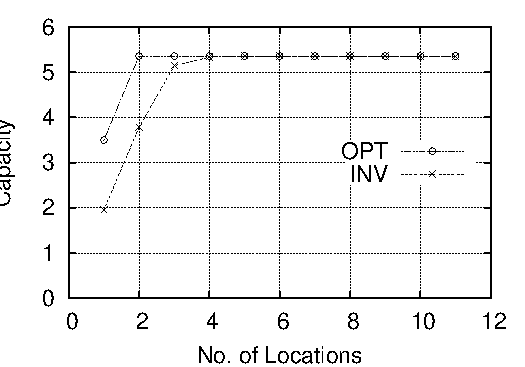
\includegraphics[scale=0.7]{final_images/G8_capacity_LP/capacity_LP.pdf}}
%	  \vspace{3in}
	  \caption{\label{fig:capacity_LP} Theoretical Capacity Increase with location diversity for an Abilene traffic matrix}
\end{figure}

When content is present at multiple location in the network, we say that the network has \emph{location diversity}.  Figure ~\ref{fig:capacity_LP} shows the increase in capacity of the network with increase in available location diversity, for two types of engineering schemes, i.e., OSPF with Inverse capacity routing(\invcap{}) and Optimal routing schemes(\opt{}). Values plotted in the graph represent the theoretical maximum capacity that can be achieved for a given degree of location diversity. These values were obtained by solving linear programs given in Appendix 9.1.  Location diversity increases the capacity of both \opt{} and \invcap{} and surprisingly  both \opt{} and \invcap{} achieve same capacity on increasing number of locations.   As can be seen from the graph, for a location diversity value of, as low as, three the maximum possible network capacity achievable by a naive OSPF inverse capacity routing scheme is almost equal to the optimal value.


We give a concrete example of BitTorrent \cite{BitTorrentRef}. BitTorrent is P2P file sharing application. A BitTorrent client, typically downloads a file from few peers simultaneously. It also keeps changing its set of peers it downloads from and continuously keeps choosing faster peers for download. If the path to one of its peers becomes congested it can switch to another peer which does does not use the congested link in its path. In this way, applications can leverage location diversity to create additional capacity in ISP networks. 



A significant fraction of internet traffic has location diversity available to it. Commercial content distribution networks (CDNs) like Akamai and cloud computing providers such as Google and Amazon have numerous servers at different geographical locations to serve content\cite{Akamai-stats,GoogleServerLocation}. Popular peer-to-peer applications such as BitTorrent and eMule also have location diversity, since each request can potentially be served by any user sharing the file. Notably, Akamai alone serves than 15-20\% of web traffic \cite{Akamai-stats} and P2P traffic is constitutes upto 65 percent of all the internet traffic\cite{ipoque}.

Since a large fraction of internet traffic has location diversity available to it, we need to examine the capacity in the ISP networks taking location diversity into account.

In this paper, we do an application centric comparison of TE schemes considering TCP throuhgput as representative of application performance. Using  \emph{ns-2} \cite{ns2}, we simulate file downloads by hundreds of users in an ISP network and compare the spectrum of TE schemes developed in the past decade . Our comparison uses ISP topology and traffic matrix data from 3 ISPs spread across US and Europe, and a realistic distribution of users access links.

The traffic engineering methods we compare are shortest path routing using link weights inverse of capacities (\invcap{}), shortest path routing using optimal weights which minimizes a link utilization based cost function (\optwt{}), offline traffic engineering using MPLS (\mplsavg{}), MLU optimal routing (\opt{})  and COPE (\cope{}), a scheme which accounts for unexpected variations in traffic. 

The main findings from our study are as follows:
\begin{enumerate}
\item 
For current ISP topologies, TMs and internet bottlenecks, TE has little value. InvCap achieve both mean and median TCP throughput within 5\% of Optimal.
\item 
MLU is a poor predictor of TCP throughput. Even a 2$\times$ difference in MLU between \opt{} and \invcap{} does not make a difference in TCP performance. \cope{} which has the MLU close to optimal has the lowest throughput among the schemes we compare
\item 
Traffic Engineering schemes which account for unexpected variations in traffic increasese the delay and reduces TCP throughput by upto 10\%.
\item
Location diversity can increase the capacity of ISP networks by 1.4$\times$. Interestingly this capacity increase can be achieved even with a small number of locations (2-4 locations).
\item
A small degree of location diversity can vanish the difference between \opt{} and other TE schemes in terms of capacity.  Even shortest path routing using \optwt{} can achieve the same capcity as \opt{}. But even with location diversity, \invcap{} has less capacity than other TE schemes.
\end{enumerate}

The rest of the paper is as follows:  Section 2 describes the experimental setup used for our comparative study. Section 3 compares different engineering schemes with respect to TCP throughput. Section 4 compares them with respect to capacity improvement and studies the impact of location diversity on capacity.  Section 5 presents related work on traffic engineering and Section 6 concludes.

%Section 7 presents a discussion and analysis of the key insights learned from the study and
